\chapter{Methodology}
The methods for this project have been developed in order to achieve the desired aims and objectives.

\section{Aims and Objectives}

The key objectives of this project are:

\begin{enumerate}
    \item To develop the necessary tools to process the raw recorded data and extract the demodulated baseband.
    \item Develop a software tool to generate an MSK waveform to allow for in depth investigation
    \item Using information extracted from the real recorded data develop a tool to simulate the atmospheric noise that appears in the real world signals.
    \item Develop an algorithm that can extract the symbols from a demodulated MSK signal.
\end{enumerate}

The key aims are:

\begin{enumerate}
    \item Investigate the signal properties from VLF transmitters around the globe listed in \ref{tab:vlftransmitters}. 
    \item Compare these properties to the simulated signals generated.
    \item Investigate how different types of noise can affect the BER associated with a particular transmission.
    \item Suggest how this BER may be improved and the impact of atmospheric noise mitigated
\end{enumerate}

\section{Implementation}
The project was implemented using python and in particular the numpy library which is off particular use for scientific computing. The reasoning for this is simply out of personal preference and the excellent facility for easy data visualisation through jupyter notebooks. 

\section{Stage 1: Development of Understanding}
The importance of developing a good simulation tool is essential in order to help assess the performance of the final algorithm as there are a lot of unknowns regarding the real data the ability to be able to create like for like simulations with known quantities is essential.
\\\\
The first stage involves an investigation into the real recording already present. In order to develop an understanding of the real data in order to help validate the later stages.
\\\\
This stage involved the basic steps of signal receptions, and developing these software tools for use later on:

\begin{enumerate}
    \item Filter

            \item The use of a rectangular filter in the frequency domain is the choice for this operation as it offers zero phase shift. Potential downsides are high frequency 'flutters' present at the temporal extremes of the data however this negates the requirement for a detailed investigation into the phase response of various filters. Working on the assumption that this rectangular filter is more or less and ideal bandpass filter.

    \item Downconvert

            Downconversion is the process of essentially removing the carrier frequency. 

    \item Low Pass Filter

            Another box car filter to extract the baseband signal

    \item Demodulate

            It is important to remember that the carrier is phase modulated, therefore
            we are interested in extracting the phase of the baseband signal. If we call baseband b(t) demodulation is shown by equations \ref{eq:instphase}
            \begin{subequations}
                \begin{equation}
                    \angle b(t) = arctan\left(\frac{Im[b(t)}{Re[b(t)]}\right) = \phi
                \end{equation}
                \begin{equation}
                    \phi = \omega t = 2\pi f
                    \label{eq:omega}
                \end{equation}
                \begin{equation}
                    \frac{d}{dt}\phi = \omega
                    \label{eq:instfeq}
                \end{equation}
                \label{eq:instphase}
            \end{subequations}
            \item Important to note that the instantaneous phase will be in the range of $pi \rightarrow -pi$, therefore it is necessary to
        \end{enumerate}


\begin{figure}[h!]
    \centering
    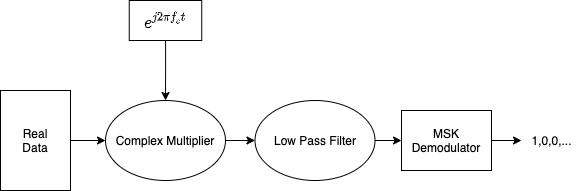
\includegraphics[width = \textwidth]{figs/method/downconversion.png}
    \caption{}
    \label{fig:my_label}
\end{figure}

The real data used consists of two seconds of data recorded using a sampling frequency of 1\si{\mega\hertz}. This stage of the exercise is to establish which of many VLF transmitters around the world are present in the recording \cite{wikipediaVLF}. The transmitters that are expected to be received are shown by table \ref{tab:vlftransmitters}.

\begin{table}[h!]
\centering
\begin{tabular}{l|l|c}
\textbf{Callsign} & \textbf{Location}    & \textbf{Centre Frequency $f_c$ [kHz]} \\
\hline 
GQD               & Anthorn, UK          & 19.6                            \\
HWU               & Saint-Assise, France & 20.9                            \\
GZQ               & Skelton, UK          & 22.1                            \\
DHO38             & Rhauderfehn, Germany & 23.4                            \\
NAA               & Cutler, Maine USA    & 24.0                             
\end{tabular}
\caption{Table of active VLF transmitters}
\label{tab:vlftransmitters}
\end{table}

This stage of the process is important to understand the nature of the real signals. The aim was to develop a full understanding of the signals that we are aiming to simulate and ultimately the real signals that the aim is to recover completely. Regarding the simulation the output of this step is to create metrics which can be used to help design, validate and improve simulation tools.

\section{Stage 2: Software Design}
In order to simulate this particular problem it has been broken into 2 separate stages.
\subsection{Carrier Generation}
The MSK carrier signal is described by equation \ref{eq:mskcarrier}. The message is split into even and odd information ie. even and odd bits, encoded as 1 or -1 corresponding to 1 or 0. These become the In Phase and Quadrature components respectively. Each bit pulses for $2T_b$ which is equivalent with the even bits pulsing on -T, T, 3T etc and the odd bits pulsing on 0, 2T, 4T etc. These odd and even signals then have to be encoded into $a_I$ and $a_Q$ these are the modulating pulse. The encoding algorithm is as follows. Figure \ref{fig:pulse} shows the resulting waveforms when $a_I$ and $a_Q$ are combined with sinusoids. Both I and Q can be considered sine waves as I simply leads Q by $\frac{\pi}{2}$ 

The important thing to note is that the phase doesn't change every symbol, but only when there is a sign change of the symbol.
These can then be used to pulse-shape, the sideband freqencies. The expected instantaneous frequency can be easily inferred from the bandwidth. Because $T_b = \frac{1}{BW}$ the frequency of the I and Q pulses is $f_{pulse} = \frac{1}{2BW}$ hence $f_{dev} = \pm\frac{f{pulse}}{2}=\pm\frac{BW}{4}$.
\begin{figure}[h!]
    \centering
    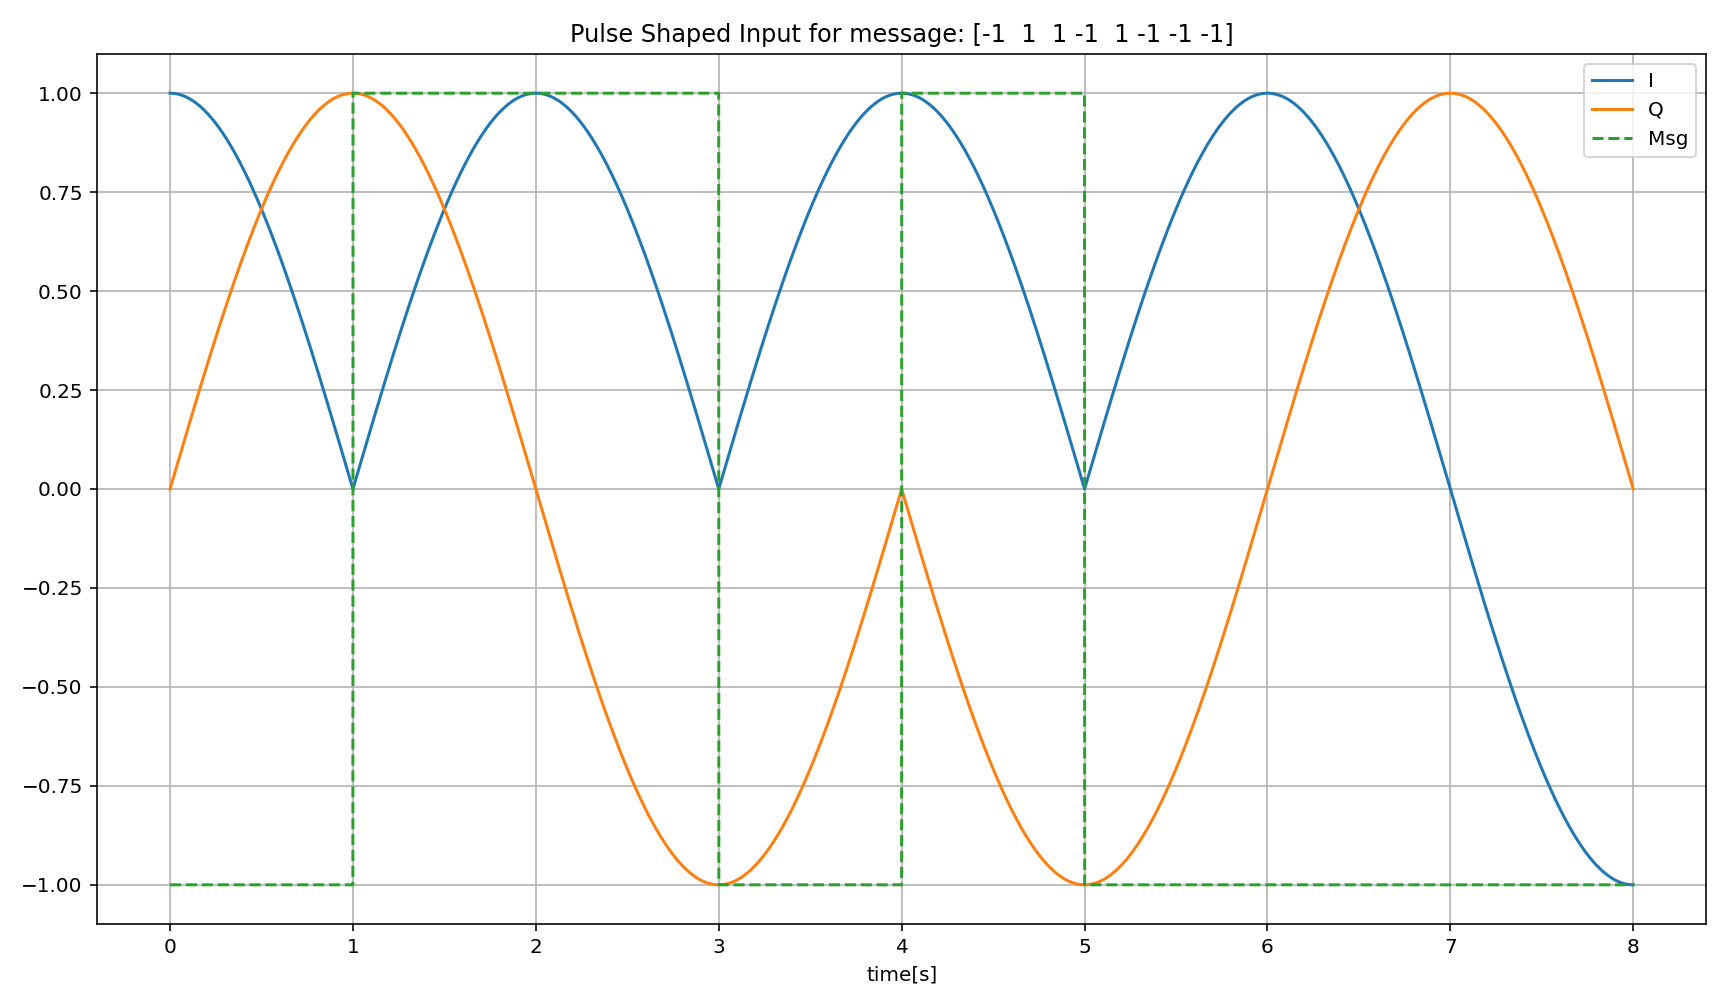
\includegraphics[width = \textwidth]{figs/method/pulseshaped.png}
    \caption{I and Q pulse weighted waveforms}
    \label{fig:pulse}
\end{figure}
\begin{equation}
s(t) = \underbrace{a_I cos\left(\frac{\pi t}{2T_b}\right)}_{\text{I Component Cosine Pulse}}\underbrace{cos(2\pi f_ct)}_{\text{Cosine Carrier}} + \underbrace{a_Qsin\left(\frac{\pi t}{2T_b}\right)}_{\text{Q Component Sine Pulse}}\underbrace{sin(2\pi f_ct)}_{\text{Sine Carrier}}
\label{eq:mskcarrier}
\end{equation}

\subsubsection{Noise Generation}
Following on from the generation of a suitable carrier signal it needs to be corrupted with noise of similar characteristics. As stated by \cite{Chrissan2000} this can be modelled using a statistical model. However as for this investigation there is data available containing an unusual amount of lightning activity this can be used to created Amplitude Probability Distribution, using the absolute amplitude of the complex trace. The complex amplitude for a signal s(t) is calculated using equation \ref{eq:complexAmp}. 
\begin{equation}
    A = \sqrt{Re[s(t)]^2 + Im[s(t)]^2}
    \label{eq:complexAmp}
\end{equation}
A discrete PDF can be developed by creating a histogram from this data using numpy's histogram method: \lstinline[language=python]{hist = np.histogram(s,bins='auto')}. This method uses the maximum of the Sturges or the Friedman-Diaconis method in order to determine bin number and width\footnote{\hyperlink{https://numpy.org/doc/stable/reference/generated/numpy.histogram.html}{https://numpy.org/doc/stable/reference/generated/numpy.histogram.html}}.
This histogram corresponds to the APD for the signal. By normalising the histogram so the histogram a cumulative distribution function can be created in order to predict an amplitude, this is simply done by using the \lstinline[language=python]{CDF = np.cumsum(hist[0])}. Once a CDF has been created, by using the numpy random library a random probability can be generated, in order to extract the corresponding amplitude value from the CDF.

In addition to developing a tool for the addition of impulsive noise. The addition 
\section{Stage 3: Algorithm Development}
Following on from the successful development of a simulation tool. The development of an algorithm to ultimately extract the symbols from the real signal, developed and tested using the simulated waveforms.

The principle of the algorithm is based on several known conditions. The process of downconversion makes the carrier frequency of the signal zero leaving only the modulating waveform. The range of the instantaneous frequency for this waveform can be used to determine the bandwidth of the signal and in turn the time per symbol $T_b$, from this the approximate number of symbols can be estimated. A symbol change ie 1 to -1 or vice versa will be observed by the signal crossing the zero axis. Using the time difference in between zero crossing the number of symbols in that interval can be determined.

\section{Stage 4: Testing and Evaluation}
The final stage of the investigation is to combine the developed tools in order to investigate the performance of the developed algorithm. The aims of this is to assess the breakdown point of the algorithm by simulating different scenarios with different types of noise. Analyse the cause of breakdown and see if further mitigation is possible.
\subsection{Investigations}
Several investigations need to be carried out in order to assess the limitations of symbol recovery. The main judge of this is the BER as previously mentioned is the number of incorrectly estimated symbols per transmission. This is shown by equation \ref{eq:ber}.
\begin{equation}
    \text{BER} = log\left(\frac{\text{Incorrect No. Bits}}{\text{Total No. Bits}}\right)
    \label{eq:ber}
\end{equation}
In order to assess the absolute performance of the symbol recovery algorithm including it's limitations, noise level need to be quantified. This is done using the signal to noise ratio, defined by equation \ref{eq:snr}, where P represents power.
\begin{subequations}
\begin{equation}
    \text{SNR} = \frac{P_{signal}}{P_{Noise}}
    \label{eq:snr}
\end{equation}
\end{subequations}

Regarding the simulated signal noise power is easy to estimate as you subtract the power of the carrier away from the power of the noise corrupted signal. However in order to estimate the SNR of the real recorded data it is necessary to make an estimate of the noise. In statistical terms the noise can be thought of as the outliers of the data. We can define the outliers as all points that lie outside of the range of the data. Equations \ref{eq:Q1} and \ref{eq:q3} are used to calculate the \nth{25} and \nth{75} percentile of the data. The interquartile range (IQR) is the difference between the two shown by equation \ref{eq:iqr}. The range limits are then determined by equations \ref{eq:upplim} and \ref{eq:lowlim}. Any data that lies outside these points is then considered noise.

\begin{subequations}
    \begin{equation}
        \text{Q1} = \text{median}\left(y_{0},y_{1},\dots,y_{\frac{N}{2}}\right)
        \label{eq:Q1}
    \end{equation}
    \begin{equation}
        \text{Q3} = \text{median}\left(y_{\frac{N}{2}},y_{\frac{N}{2}+1},\dots,y_{N}\right)
        \label{eq:q3}
    \end{equation}
    \begin{equation}
        IQR = Q3 - Q1
        \label{eq:iqr}
    \end{equation}
    \begin{equation}
        \text{Lim}_{\text{upper}} = Q3 + k IQR
        \label{eq:upplim}
    \end{equation}
    \begin{equation}
        \text{Lim}_{\text{lower}} = Q1 - k IQR
        \label{eq:lowlim}
    \end{equation}
\end{subequations}

\section{Assumptions}
\begin{enumerate}
    \item The algorithm is implemented on a signal irrespective of phase synchronisation.
    \item All noise generated will have only a real component
    \item 
\end{enumerate}
